\documentclass[aspectratio=169,10pt]{beamer}

% --- Theme and layout ---
\usetheme{Darmstadt}
\usecolortheme{default}
\usefonttheme{default}
\usefonttheme[onlymath]{serif}
\setbeamertemplate{navigation symbols}{}
\setbeamertemplate{footline}{}
\setbeamertemplate{caption}[numbered]
\setbeamertemplate{blocks}[rounded][shadow=true]
\usepackage{tikz}
\usetikzlibrary{arrows.meta,positioning}

\definecolor{raceblue}{RGB}{35,110,180}
\definecolor{othergray}{RGB}{215,220,225}

% Slightly reduce spacing around displayed equations
\AtBeginDocument{
  \setlength{\abovedisplayskip}{5pt}
  \setlength{\belowdisplayskip}{5pt}
  \setlength{\abovedisplayshortskip}{3pt}
  \setlength{\belowdisplayshortskip}{3pt}
}



\usepackage[T1]{fontenc}
\usepackage{lmodern}
\usepackage{amsmath,amssymb}
\usepackage{tikz}
\usepackage{pgfplots}
\usetikzlibrary{arrows.meta,positioning}
\pgfplotsset{compat=1.18}

\definecolor{raceblue}{RGB}{35,110,180}
\definecolor{othergray}{RGB}{215,220,225}

\setbeamercolor{structure}{fg=raceblue}
\setbeamertemplate{navigation symbols}{}

% Left and right margins
\setbeamersize{
    text margin left=0.8cm,
    text margin right=0.8cm
}

% Space above and below each slide title
\addtobeamertemplate{frametitle}
    {\vspace*{0.05cm}}
    {\vspace*{0.02cm}}

% Reserve bottom space and keep page numbers away from the edge
\setbeamertemplate{footline}{%
    \leavevmode
    \hbox{%
        \begin{beamercolorbox}[
            wd=\paperwidth,
            ht=0.22cm,
            dp=0.12cm,
            right
        ]{normal text}%
            \usebeamerfont{page number in head/foot}%
            \insertframenumber\hspace*{0.8cm}%
        \end{beamercolorbox}%
    }%
}

% Two equally populated neighborhoods.
% Argument 1: number of blue dots in the upper neighborhood.
% Argument 2: number of blue dots in the lower neighborhood.
% Arguments 3 and 4: neighborhood group shares.
\newcommand{\citydiagram}[4]{%
\begin{tikzpicture}[x=0.43cm,y=0.43cm]
    \draw[rounded corners,gray]
        (-0.6,-0.6) rectangle (4.6,1.6);
    \draw[rounded corners,gray]
        (-0.6,-3.6) rectangle (4.6,-1.4);

    \foreach \x in {0,...,4}{
        \foreach \y in {0,1}{
            \fill[othergray] (\x,\y) circle (0.19);
            \fill[othergray] (\x,\y-3) circle (0.19);
        }
    }

    \ifnum#1>0
        \foreach \i in {1,...,#1}{
            \fill[raceblue] ({\i-1},1) circle (0.19);
        }
    \fi
    \ifnum#2>0
        \foreach \i in {1,...,#2}{
            \fill[raceblue] ({\i-1},-2) circle (0.19);
        }
    \fi

    \node[right,font=\scriptsize] at (4.8,0.5)
        {$r_1=#3$};
    \node[right,font=\scriptsize] at (4.8,-2.5)
        {$r_2=#4$};

    \draw[<->,>=Stealth,gray,thick]
        (2,-0.65) -- (2,-1.35);
\end{tikzpicture}%
}
% --- Color palette ---
\definecolor{MyNavy}{RGB}{25,58,86}
\definecolor{MyTeal}{RGB}{43,119,125}
\definecolor{MyLightBlue}{RGB}{232,239,244}

\setbeamercolor{normal text}{fg=black,bg=white}
\setbeamercolor{structure}{fg=MyNavy}
\setbeamercolor{frametitle}{fg=white,bg=MyNavy}
\setbeamercolor{title}{fg=white,bg=MyNavy}
\setbeamercolor{titlelike}{fg=white,bg=MyNavy}
\setbeamercolor{section in head/foot}{fg=white,bg=MyNavy}
\setbeamercolor{subsection in head/foot}{fg=white,bg=MyTeal}
\setbeamercolor{block title}{fg=white,bg=MyNavy}
\setbeamercolor{block body}{fg=black,bg=MyLightBlue}
\setbeamercolor{alerted text}{fg=MyTeal}
\setbeamercolor{author}{fg=black}
\setbeamercolor{date}{fg=black}
\setbeamercolor{institute}{fg=black}

% --- Packages ---
\usepackage{amsmath,amssymb,amsbsy}
\usepackage{graphicx}
\usepackage{url}
% \usepackage{biblatex} % Unused: no bibliography commands in this deck.
\usepackage{algorithm}
\usepackage[noend]{algpseudocode}
\usepackage{siunitx}
\usepackage{tikz}
\usepackage{appendixnumberbeamer}

% Uncomment if ref.bib exists in your Overleaf project.
% \addbibresource{ref.bib}

% --- Presentation metadata ---
\title{Comparing Segregation Metrics}
\author[Che, Klein, Pan, Sun]{Derek Che, Zachary Klein, Michelle Pan, Sophia Sun}
\date{\today}


% Fit long display equations within the current column without changing them.
\usepackage{adjustbox}
\long\def\[#1\]{%
  \begin{equation*}
    \begin{adjustbox}{max width=0.98\linewidth}
      $\displaystyle #1$
    \end{adjustbox}
  \end{equation*}%
}
\setbeamerfont{frametitle}{size=\large}

\begin{document}
\addtobeamertemplate{block begin}
    {\setlength\abovedisplayskip{0pt}}{}


% Slide 1: Title
\begin{frame}[plain,shrink=0]
\centering
\vspace{0.75cm}
\begin{minipage}{0.88\paperwidth}
\begin{beamerboxesrounded}[upper=block title,lower=block title,shadow=true]{}
    \centering
    \vspace{0.15cm}
    {\usebeamerfont{title}\color{white}Comparing Segregation Metrics\par}
    \vspace{0.15cm}
\end{beamerboxesrounded}
\end{minipage}

\vspace{0.65cm}
{\normalsize Derek Che, Zachary Klein, Michelle Pan, Sophia Sun\par}
\vspace{0.5cm}
{\normalsize \insertdate\par}
\vspace{0.4cm}
    \includegraphics[width=0.18\textwidth,height=1.45cm,keepaspectratio]{Columbia shield.png}\par
\vspace{0.4cm}
{\small APMA E4903: Seminar in Applied Mathematics\par}
\end{frame}

% Slide 2: Presentation Outline
\begin{frame}[shrink=0]{Presentation Outline}
\begin{enumerate}
    \item Introduction and Motivation
    \item Background: Existing Segregation Measures
    \item Our Modified Segregation Metric
    \item Analysis and Results
    \item Discussion and Future Directions
    \item Conclusion
\end{enumerate}
\end{frame}

% Slide 3: Meet the Presenters
\begin{frame}[shrink=0]{Meet the Presenters}
\begin{columns}[T,onlytextwidth]
\begin{column}{0.48\textwidth}
\textbf{Derek Che}

Academic interests: TBD

Project contribution: TBD

\vspace{0.5cm}
\textbf{Zachary Klein}

Academic interests: Gambling Theory

Project contribution: TBD
\end{column}
\begin{column}{0.48\textwidth}
\textbf{Michelle Pan}

Academic interests: TBD

Project contribution: TBD

\vspace{0.5cm}
\textbf{Sophia Sun}

Academic interests: TBD

Project contribution: TBD
\end{column}
\end{columns}
\end{frame}

% Slide 4: Primary References
\begin{frame}[shrink=0]{Primary References}
\small
\begin{enumerate}
    \item Echenique, F., and Fryer, R. G., Jr. (2007).
    ``A Measure of Segregation Based on Social Interactions.''
    \textit{The Quarterly Journal of Economics}, 122(2), 441--485.
    \item Coleman, J. S. (1958).
    ``Relational Analysis: The Study of Social Organizations with Survey Methods.''
    \textit{Human Organization}, 17(4), 28--36.
    \href{https://doi.org/10.17730/humo.17.4.q5604m676260q8n7}{doi:10.17730/humo.17.4.q5604m676260q8n7}.
    \item Bordenave, C., Caputo, P., and Chafa\"i, D. (2012).
    ``Circular Law Theorem for Random Markov Matrices.''
    \textit{Probability Theory and Related Fields}, 152, 751--779.
    \href{https://arxiv.org/abs/0808.1502}{arXiv:0808.1502}.
\end{enumerate}
\end{frame}

\section{Introduction}

% Slide 3: Motivation
\begin{frame}[shrink=0]{Why Study Segregation?}
    \begin{itemize}
        \item Segregation shapes opportunities for
        social interaction.

        \item Traditional measures often rely on
        geographic boundaries.

        \item Geographic proximity does not always
        imply accessibility.

        \item Transportation may connect communities
        that are otherwise geographically separated.
    \end{itemize}
\end{frame}

% Slide 4: Research question
\begin{frame}[shrink=0]{Our Research Question}
    \begin{block}{Main Question}
        How does incorporating transportation
        accessibility change our measurement
        of segregation?
    \end{block}

    \vspace{0.3cm}

    \begin{itemize}
        \item Can travel time and monetary cost
        improve measures of social connectivity?

        \item How do train lines affect measured
        segregation between neighborhoods?

        \item How do our results compare with
        existing segregation measures?
    \end{itemize}
\end{frame}



% =====================================================
% PERRON--FROBENIUS THEOREM
% =====================================================

\subsection{Perron--Frobenius Theorem}

% Slide 1
\begin{frame}[shrink=0]{Perron--Frobenius Theorem}
\small

Let $A\in\mathbb{R}^{n\times n}$ be strictly positive,
meaning $a_{ij}>0$ for all $i,j$.

\begin{block}{Proposition 5.1: Perron Root}
There exists a positive eigenvalue $r=\rho(A)$,
and every other eigenvalue $\lambda$ satisfies
\[
|\lambda|<r.
\]
\end{block}

\begin{block}{Proposition 5.2: Positive Eigenvectors}
There exist strictly positive vectors $v,w$ with
\[
Av=rv,\qquad w^TA=rw^T.
\]
\end{block}

\begin{block}{Proposition 5.3: Simplicity}
The eigenvalue $r$ has algebraic multiplicity one.
\end{block}

\end{frame}



\begin{frame}[shrink=0]{Proposition 5.1: Positive Spectral Radius}
\small

Recall that the spectral radius of $A$ is
\[
\rho(A)=\max\{|\lambda|:
\lambda\text{ is an eigenvalue of }A\}.
\]

Let $c=\min_{i,j}a_{ij}>0$, and let $J$
denote the all-ones matrix.

Since every entry of $A$ is at least $c$,
\[
0\leq cJ\leq A.
\]

\begin{block}{Spectral-Radius Monotonicity}
For nonnegative matrices $B\leq C$
(entrywise), we have
\[
\rho(B)\leq\rho(C).
\]
\end{block}

Applying this property to $cJ$ and $A$ gives
\[
\boxed{\rho(A)\geq\rho(cJ)=nc>0.}
\]

Thus, the spectral radius of $A$ is positive.

\end{frame}

% Slide 3
\begin{frame}[shrink=0]{Proposition 5.1: Why Monotonicity Holds}
\small

Suppose $0\leq B\leq C$ entrywise.

Because both matrices are nonnegative,
multiplication preserves the inequalities:
\[
0\leq B^k\leq C^k
\qquad(k\geq1).
\]

Using the infinity norm,
\[
\|B^k\|_\infty\leq\|C^k\|_\infty.
\]

By Gelfand's formula,
\[
\rho(B)=\lim_{k\to\infty}
\|B^k\|_\infty^{1/k}.
\]

Consequently,
\[
\boxed{\rho(B)\leq\rho(C).}
\]

\begin{block}{Application}
Taking $B=cJ$ and $C=A$ proves
that $\rho(A)>0$.
\end{block}

\end{frame}


% Slide 4
\begin{frame}[shrink=0]{Proposition 5.1: Strict Dominance (I)}
\small

Normalize $A$ by its spectral radius:
\[
M=\frac{A}{\rho(A)},\qquad \rho(M)=1.
\]

Choose an eigenvalue $\mu$ of $M$ satisfying
$|\mu|=1$.

We want to show that $\mu=1$.

Suppose instead that $\mu\neq1$.
Choose an integer $m\geq1$ such that
\[
\operatorname{Re}(\mu^m)<0.
\]

Since $M>0$, we also have $M^m>0$.

For sufficiently small $\varepsilon>0$,
define
\[
T=M^m-\varepsilon I\geq0.
\]

\begin{block}{Key Observation}
Because $\mu^m$ is an eigenvalue of $M^m$,
the number $\mu^m-\varepsilon$ is an
eigenvalue of $T$.
\end{block}

\end{frame}




% Slide 5
\begin{frame}[shrink=0]{Proposition 5.1: Strict Dominance (II)}
\small

From the previous slide,
$\mu^m-\varepsilon$ is an eigenvalue of $T$.

Since $|\mu|=1$ and
$\operatorname{Re}(\mu^m)<0$,
\[
\begin{aligned}
|\mu^m-\varepsilon|^2
&=|\mu^m|^2
  -2\varepsilon\operatorname{Re}(\mu^m)
  +\varepsilon^2\\
&=1-2\varepsilon\operatorname{Re}(\mu^m)
  +\varepsilon^2\\
&>1.
\end{aligned}
\]

Thus
\[
\rho(T)\geq|\mu^m-\varepsilon|>1.
\]

\begin{block}{Contradiction}
But $0\leq T\leq M^m$, so monotonicity gives
\[
\rho(T)\leq\rho(M^m)=1.
\]
\end{block}


Thus $1$ is the only eigenvalue of $M$
with modulus one.

Since $\rho(M)=1$, such an eigenvalue
must exist. Hence $1$ is an eigenvalue
of $M$, so $r=\rho(A)>0$ is an eigenvalue
of $A$.

Every other eigenvalue $\lambda$ of $A$
therefore satisfies $|\lambda|<r$.


\end{frame}



% Proposition 5.2 -- Slide 1
\begin{frame}[shrink=0]{Proposition 5.2: Positive Eigenvectors (I)}
\small

By Proposition 5.1, $r=\rho(A)>0$ is a real
eigenvalue. Choose a nonzero real eigenvector $x$:
\[
Ax=rx.
\]

Define $y=|x|$, taking absolute values
componentwise. Then $y\geq 0$ and $y\neq 0$.

Since $A$ has strictly positive entries,
the triangle inequality gives
\[
Ay\geq |Ax|=r|x|=ry.
\]

\begin{block}{Goal}
We want to show that equality holds:
\[
Ay=ry.
\]
This would give us a nonnegative eigenvector.
\end{block}

\end{frame}


% Proposition 5.2 -- Slide 2
\begin{frame}[shrink=0]{Proposition 5.2: Positive Eigenvectors (II)}
\small

Suppose $Ay\geq ry$ is strict in at least
one coordinate.

Define
\[
d=Ay-ry\geq0,\qquad d\neq0.
\]

Because $A>0$ and $d$ is nonnegative
and nonzero, every component of $Ad$
is strictly positive:
\[
Ad>0.
\]

Multiplying $Ay=ry+d$ by $A$ gives
\[
A^2y=rAy+Ad>rAy.
\]

Now set $v=Ay>0$. Consequently,
\[
\boxed{Av>rv.}
\]

\end{frame}


% Proposition 5.2 -- Slide 3
\begin{frame}[shrink=0]{Proposition 5.2: Positive Eigenvectors (III)}
\small

We have $v>0$ and $Av>rv$.

Define
\[
q=\min_i\frac{(Av)_i}{v_i}.
\]

Since the inequality is strict in every
coordinate,
\[
q>r,\qquad Av\geq qv.
\]


Repeated multiplication by $A$ gives
\[
A^kv\geq q^kv.
\]

Taking infinity norms,
\[
\|A^k\|_\infty
\geq
\frac{\|A^kv\|_\infty}{\|v\|_\infty}
\geq q^k.
\]

By Gelfand's formula,
\[
\rho(A)=\lim_{k\to\infty}
\|A^k\|_\infty^{1/k}\geq q>r.
\]

This contradicts $\rho(A)=r$.

\end{frame}


% Proposition 5.2 -- Slide 4
\begin{frame}[shrink=0]{Proposition 5.2: Positive Eigenvectors (IV)}
\small

The contradiction shows that our
original inequality cannot be strict.
Therefore,
\[
Ay=ry.
\]

Since $A>0$ and $y\geq0$ is nonzero,
we know $Ay>0$.

Because $r>0$, the equation $Ay=ry$
implies $y>0$.

\begin{block}{Positive Right and Left Eigenvectors}
We have obtained a positive right
eigenvector $y>0$ satisfying $Ay=ry$.

Since $A^T>0$ and $\rho(A^T)=r$,
the same argument gives $w>0$ with
\[
A^Tw=rw
\quad\Longleftrightarrow\quad
w^TA=rw^T.
\]
\end{block}

\end{frame}


% Proposition 5.3 -- Geometric Simplicity
\begin{frame}[shrink=0]{Proposition 5.3: Geometric Simplicity}
\small

By Proposition 5.2, there exists $x>0$
such that $Ax=rx$.

Let $y$ be another real eigenvector
corresponding to $r$, so $Ay=ry$.

Define
\[
t=\max_i\frac{y_i}{x_i},
\qquad z=tx-y.
\]

By construction, $z\geq0$, and at least
one component of $z$ is zero.

Since $Ax=rx$ and $Ay=ry$,
\[
Az=tAx-Ay=r(tx-y)=rz.
\]

If $z\neq0$, then $A>0$ implies $Az>0$.
But $rz$ has a zero component,
giving a contradiction.

\begin{block}{Conclusion}
Thus $z=0$, so $y=tx$.
The result extends to complex eigenvectors
by considering real and imaginary parts.

Therefore,
\[
\boxed{\dim\ker(A-rI)=1.}
\]
\end{block}

\end{frame}


% Proposition 5.3 -- Algebraic Simplicity (I)
\begin{frame}[shrink=0]{Proposition 5.3: Algebraic Simplicity (I)}
\small

By Proposition 5.2, there exist positive
right and left eigenvectors $x,w>0$ such that
\[
Ax=rx,\qquad A^Tw=rw.
\]

Suppose, for contradiction, that $r$
has algebraic multiplicity greater than one.

We already proved that its eigenspace is
one-dimensional:
\[
\dim\ker(A-rI)=1.
\]

Therefore, there exists a generalized
eigenvector $u$ satisfying
\[
(A-rI)u=x.
\]

\begin{block}{Key Idea}
We will multiply this equation by the
positive left eigenvector $w^T$ to
obtain a contradiction.
\end{block}

\end{frame}


\begin{frame}[shrink=0]{Proposition 5.3: Algebraic Simplicity (II)}
\small

From the previous slide, we have
\[
(A-rI)u=x.
\]

Multiplying by the left eigenvector $w^T$ gives
\[
w^T(A-rI)u=w^Tx.
\]

Since $w^TA=rw^T$, we know
\[
w^T(A-rI)=w^TA-rw^T=0.
\]

Therefore, the left-hand side is zero,
while the right-hand side is positive.

\begin{block}{Contradiction}
\[
\boxed{0=w^Tx>0.}
\]

This is impossible because $w,x>0$,
so their dot product is strictly positive.

Thus, $r$ must be algebraically simple.
\end{block}

\end{frame}

%END OF PF

\subsection{Motivation and Research Goals}
\begin{frame}[shrink=0]{Limitations of Existing Measures}
\begin{itemize}
    \item Geographic partitions may not accurately
    represent opportunities for social interaction.

    \item Echenique and Fryer's SSI addresses this
    by considering networks of social connections.

    \item However, physical proximity does not
    necessarily imply accessibility.

    \item Transportation networks may connect distant
    neighborhoods or leave nearby areas isolated.
\end{itemize}
\end{frame}

\begin{frame}[shrink=0]{Our Research Goal}
\begin{itemize}
    \item Incorporate transportation accessibility
    into the measurement of segregation.

    \item Account for travel time and monetary cost
    when measuring connections between areas.

    \item Compare segregation with and without
    transportation connections.

    \item Investigate how train lines may connect
    otherwise separated communities.
\end{itemize}
\end{frame}

\section{Our Model}

\begin{frame}[shrink=0]{Modeling Transportation Accessibility}

We define a social connection weight between
nodes $i$ and $j$:

\[
f(i \to j) = e^{-\beta C_{ij}}
\]

where

\[
C_{ij} =
\max\left\{
c_0,\,
\min_{m \in \mathcal{M}}
[p_{ij}^{m}+\omega t_{ij}^{m}]
\right\}
\]

\begin{itemize}
    \item $p_{ij}^{m}$: monetary travel cost
    \item $t_{ij}^{m}$: travel time
    \item $\omega$: monetary value of time
    \item $\beta$: sensitivity to travel cost
    \item $c_0$: minimum local encounter cost
\end{itemize}

\end{frame}

% ========================================
% ECHENIQUE--FRYER ORIGINAL SSI
% ========================================
\begin{frame}[shrink=0]{Echenique--Fryer (2007): Original SSI}
\small

\begin{block}{Original Method}
\begin{itemize}
    \item Construct a social-interaction matrix, retaining
    same-group interaction weights.

    \item For residential segregation, treat census blocks
    within 1 km as neighbors, assigning weight $1/d_i$
    to each of node $i$'s neighbors.

    \item For each same-group connected component $C$,
    measure segregation using the spectral radius:
    \[
       \boxed{S_r(C)=\rho\bigl(B_r|_C\bigr).}
    \]
\end{itemize}
\end{block}

\begin{block}{Limitations of Their Residential Application}
\begin{itemize}
    \item Geographic proximity alone does not capture
    travel time, monetary cost, or transit connectivity.

    \item Equal neighbor weights overlook differences in
    accessibility, and the block-level implementation
    does not explicitly account for population density.
\end{itemize}
\end{block}

\end{frame}

\begin{frame}[shrink=0]{Our Modified Segregation Metric}

For a racial group $r$, define the interaction matrix
$A$ with the entries

\[
a_{ij} =
\frac{
D(j)f(i\to j)\mathbb{P}_j(r)
}{
\sum_{k=1}^{n}f(i\to k)D(k)
}
\]

where

\begin{itemize}
    \item $D(j)$: population at node $j$
    \item $\mathbb{P}_j(r)$: proportion of group $r$
    at node $j$
    \item $f(i\to j)$: transportation-based
    connection weight
\end{itemize}

The segregation index is the spectral radius:

\[
\boxed{S_r = \rho(A)}
\]

\end{frame}

\subsection{Monotonicity and Linearity}

% ----------- MONOTONICITY -----------
\begin{frame}[shrink=0]{Monotonicity: Statement}
\small
For a fixed group $r$, recall that our segregation index is
\[
S_r(A)=\rho(A), \qquad
 a_{ij}=\frac{D(j)f(i\to j)P_j(r)}{\sum_{k=1}^{n}f(i\to k)D(k)}.
\]
\begin{block}{Monotonicity}
Let $A$ and $B$ be nonnegative interaction matrices on the same
nodes. If $B\ge A$ entrywise, then
\[
\boxed{\rho(B)\ge\rho(A).}
\]
\end{block}
\medskip
\textbf{Interpretation:} Strengthening same-group interaction
intensities without weakening any of them cannot reduce the index.
\end{frame}

\begin{frame}[shrink=0]{Monotonicity: Proof}
\small
Assume $A$ is irreducible. By Perron--Frobenius, there is a
positive eigenvector $v>0$ with
\[
Av=\lambda_Av,\qquad \lambda_A=\rho(A).
\]
Since $B\ge A$ entrywise and $v>0$,
\[
Bv\ge Av=\lambda_Av.
\]
Thus, for every $i$,
\[
\frac{(Bv)_i}{v_i}\ge\lambda_A
\quad\Longrightarrow\quad
\min_i\frac{(Bv)_i}{v_i}\ge\lambda_A.
\]
\begin{block}{Collatz--Wielandt Bound}
\[
\boxed{\rho(B)\ge\min_i\frac{(Bv)_i}{v_i}
\ge\lambda_A=\rho(A).}
\]
\end{block}
\end{frame}

\begin{frame}[shrink=0]{Strict Monotonicity}
\small
Suppose additionally that $B\ne A$. Since $A$ is irreducible
and $B\ge A$, $B$ is also irreducible.

Let $u>0$ be a \emph{left} Perron eigenvector of $B$ and
$v>0$ a right Perron eigenvector of $A$:
\[
u^TB=\rho(B)u^T,\qquad Av=\rho(A)v.
\]
Because $B-A\ge0$ has at least one positive entry,
\[
u^T(B-A)v>0.
\]
Substituting the eigenvector equations,
\[
\bigl(\rho(B)-\rho(A)\bigr)u^Tv>0.
\]
\begin{block}{Conclusion}
Since $u^Tv>0$, \(\boxed{\rho(B)>\rho(A)}\).
\end{block}
\end{frame}

% ----------- LINEARITY -----------
\begin{frame}[shrink=0]{Linearity: Interaction Weights}
\small
Define the probability of an encounter from node $i$ occurring
at node $j$, regardless of group:
\[
H(i\to j)=\frac{D(j)f(i\to j)}
{\sum_{k=1}^{n}f(i\to k)D(k)}.
\]
By construction,
\[
\sum_{j=1}^{n}H(i\to j)=1.
\]
Only a fraction $P_j(r)$ of node $j$ belongs to group $r$, so
\[
\boxed{a_{ij}=H(i\to j)P_j(r).}
\]
\begin{block}{Key Idea}
Each destination's contribution depends on both its accessibility
and its group-$r$ population share.
\end{block}
\end{frame}

\begin{frame}[shrink=0]{Linearity: From Eigenvectors to Scores}
\small
Let $\lambda=\rho(A)>0$ and let $v>0$ satisfy $Av=\lambda v$.
For each node $i$,
\[
\lambda v_i=\sum_{j=1}^{n}a_{ij}v_j
\quad\Longrightarrow\quad
v_i=\frac{1}{\lambda}\sum_{j=1}^{n}a_{ij}v_j.
\]
Define the group-$r$ population $N_j=D(j)P_j(r)$ and the
population-weighted eigenvector mean
\[
\bar v_N=\frac{\sum_jN_jv_j}{\sum_jN_j}.
\]
The individual score is $\hat S_i=\lambda v_i/\bar v_N$.
Since $c=\lambda/\bar v_N$ is constant, $\hat S_i=cv_i$.
\begin{block}{Multiply the Eigenvector Equation by $c$}
\[
\boxed{\hat S_i=\frac{1}{\lambda}
\sum_{j=1}^{n}a_{ij}\hat S_j.}
\]
\end{block}
\end{frame}

\begin{frame}[shrink=0]{Linearity: Final Result}
\small
Substitute $a_{ij}=H(i\to j)P_j(r)$ into the previous result:
\begin{block}{Linearity Under Population-Weighted Interactions}
\[
\boxed{\hat S_i=\frac{1}{\lambda}\sum_{j=1}^{n}
H(i\to j)P_j(r)\hat S_j.}
\]
\end{block}
\medskip
\textbf{Interpretation:} A person's segregation score is a
linear combination of the scores of their potential same-group
contacts. Each contribution reflects
\begin{itemize}
\item how likely the person is to encounter node $j$, and
\item how likely the encountered person is to belong to group $r$.
\end{itemize}
\medskip
\footnotesize\emph{Note:} The coefficients are not necessarily
normalized to sum to one, so this is a linear combination,
not always a weighted average.
\end{frame}


\section{The Index as a Random Walk}
 
% ---------------------------------------------------------------------
% 1. Hook
% ---------------------------------------------------------------------
\begin{frame}[shrink=0]{Does the Index Depend on How We Draw the Map?}
\begin{itemize}
    \item Our nodes are census units: someone else drew the boundaries.
    \item If splitting a block in two changes the index, we are measuring
    \alert{cartography}, not segregation.
\end{itemize}
 
\vspace{0.3cm}
\begin{block}{Claim}
If a node is split into two \emph{co-located} pieces, the group index
is unchanged and every person keeps their individual index.
\end{block}
 
\vspace{0.2cm}
\begin{block}{Why, in one sentence}
The index measures a random walk over \emph{people}. Splitting a node
relabels people; it does not change who meets whom.
\end{block}
% SAY: The rest of my section cashes out this one sentence.
\end{frame}
 
% ---------------------------------------------------------------------
% 2. The matrix as a probability
% ---------------------------------------------------------------------
\begin{frame}[shrink=0]{Reading $A$ as an Encounter Probability}
Race-$r$ headcount and normalizer:
\[
N_j = D(j)\,\mathbb{P}_j(r), \qquad
Z_i = \sum_{k} f(i\to k)\,D(k).
\]
Then
\[
a_{ij} = \frac{f(i\to j)\,N_j}{Z_i}
\]
\[
\phantom{a_{ij}} = \Pr\big(\text{person at } i \text{ draws a race-}r
\text{ partner at } j\big).
\]
\begin{itemize}
    \item Row sum $F_i = \sum_j a_{ij} \le 1$: probability of drawing
    \emph{any} race-$r$ partner. So $A$ is substochastic.
    \item Restrict to $V_r = \{i : N_i > 0\}$, $d = |V_r|$
    (we reserve $n$ for steps of a walk).
\end{itemize}
% SAY: Same formula as before (D(j) P_j(r) = N_j), read as a probability.
%      The denominator counts everyone; the numerator only race-r people.
\end{frame}
 
% ---------------------------------------------------------------------
% 3. Group and individual index
% ---------------------------------------------------------------------
\begin{frame}[shrink=0]{Group and Individual Index}
\textbf{Assumptions:} $f(i\to i) > 0$ and $A$ irreducible on $V_r$.
For us automatic: $f = e^{-\beta C} > 0$ whenever a route exists.
 
\vspace{0.2cm}
By Perron--Frobenius: $\lambda = \rho(A) > 0$, with $v > 0$,
$Av = \lambda v$, unique up to scale.
 
\begin{block}{Definition}
\[
\text{group index } \lambda \;(= S_r), \qquad
\hat s_i = \lambda\,\frac{v_i}{\bar v_N}, \quad
\bar v_N = \frac{\sum_j N_j v_j}{\sum_j N_j}.
\]
\end{block}
\begin{itemize}
    \item $\bar v_N$ averages over \alert{people}, not nodes. Then
    $\dfrac{\sum_i N_i \hat s_i}{\sum_i N_i} = \lambda$:
    the group index is the average person's index.
    \item Echenique--Fryer average over nodes. Same thing when each
    node is one person ($N_j = 1$).
\end{itemize}
% SAY: Hand-off from PF: we now have lambda and v > 0. Plant the
%      people-vs-nodes normalization; it pays off at the end.
\end{frame}
 
% ---------------------------------------------------------------------
% 4. The encounter walk
% ---------------------------------------------------------------------
\begin{frame}[shrink=0]{The Encounter Walk}
\begin{columns}[T,onlytextwidth]
\begin{column}{0.42\textwidth}
\centering
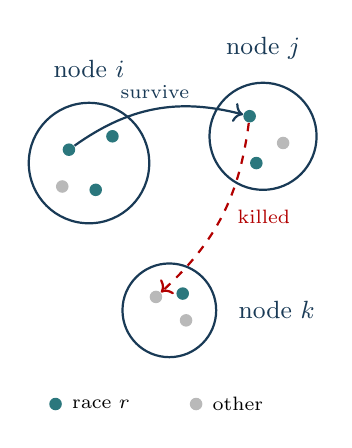
\begin{tikzpicture}[scale=0.85,
    p/.style={circle,fill=MyTeal,inner sep=1.6pt},
    o/.style={circle,fill=gray!55,inner sep=1.6pt}]
    \draw[MyNavy,thick] (0,0) circle (0.9) node[above=0.95cm] {\small node $i$};
    \draw[MyNavy,thick] (2.6,0.4) circle (0.8) node[above=0.85cm] {\small node $j$};
    \draw[MyNavy,thick] (1.2,-2.2) circle (0.7) node[right=0.75cm] {\small node $k$};
    \node[p] (x) at (-0.3,0.2) {};
    \node[p] at (0.35,0.4) {}; \node[p] at (0.1,-0.4) {};
    \node[o] at (-0.4,-0.35) {};
    \node[p] (y) at (2.4,0.7) {}; \node[o] at (2.9,0.3) {};
    \node[p] at (2.5,0.0) {};
    \node[o] (z) at (1.0,-2.0) {}; \node[o] at (1.45,-2.35) {};
    \node[p] at (1.4,-1.95) {};
    \draw[->,thick,MyNavy] (x) to[bend left=25] node[above]{\scriptsize survive} (y);
    \draw[->,thick,red!70!black,dashed] (y) to[bend left=20] node[right,xshift=2pt]{\scriptsize killed} (z);
    \node[p,label=right:{\scriptsize race $r$}] at (-0.5,-3.6) {};
    \node[o,label=right:{\scriptsize other}] at (1.6,-3.6) {};
\end{tikzpicture}
\end{column}
\begin{column}{0.56\textwidth}
\small
A walker moves through \alert{people}, not nodes.
\begin{enumerate}
    \item From person $X_t$ at node $\ell(X_t)$, draw person $q$ with
    \[
    K(X_t, q) = \frac{f\big(\ell(X_t)\to\ell(q)\big)}{Z_{\ell(X_t)}}.
    \]
    \item If $q$ is not race $r$, the walk is \emph{killed}.
    Otherwise $X_{t+1} = q$.
\end{enumerate}
$T$ = killing time.
 
\vspace{0.2cm}
\textbf{Key:} $K$ depends on $q$ only through its location $\ell(q)$.
\end{column}
\end{columns}
% SAY: K is a genuine Markov transition matrix on people (rows sum to 1
%      by the definition of Z). Everyone at a node looks identical to the
%      walker -- that is the property the whole proof runs on.
\end{frame}
 
% ---------------------------------------------------------------------
% 5. Backward equation
% ---------------------------------------------------------------------
\begin{frame}[shrink=0]{Backward Equation: Survival Is $A^n\mathbf{1}$}
Let $\sigma_i(n) = \Pr(T > n \mid X_0 \text{ at node } i)$.
 
\vspace{0.15cm}
\textbf{Condition on the first step} (backward Kolmogorov):
\[
g_n(p) = \sum_{q \text{ race } r} K(p,q)\, g_{n-1}(q), \qquad g_0 \equiv 1.
\]
Group by node (the $N_j$ race-$r$ people at $j$ are equally likely):
\[
\sum_{q \text{ at } j} K(p,q) = \frac{f(i\to j)\,N_j}{Z_i} = a_{ij}
\quad\Longrightarrow\quad
\boxed{\sigma(n) = A^n\mathbf{1}}
\]
\begin{block}{Interpretation}
$\sigma_i(n)$ = probability of $n$ consecutive own-race encounters
starting from someone at $i$: \alert{$n$-th order segregation}.
$\sigma(1) = F$. With $N_j = 1$, this is Echenique--Fryer's
``higher-order segregation,'' made precise.
\end{block}
% SAY: "Backward" because we condition on where the walker goes next
%      and look at the future from there.
\end{frame}
 
% ---------------------------------------------------------------------
% 6. From A to a genuine chain
% ---------------------------------------------------------------------
\begin{frame}[shrink=0]{From $A$ to a Genuine Markov Chain}
$A$ is substochastic (the walk dies), so Markov chain limit theorems do
not apply to it directly. Use $(\lambda, v)$:
\[
P_{ij} = \frac{a_{ij}\, v_j}{\lambda\, v_i}, \qquad
\sum_j P_{ij} = \frac{(Av)_i}{\lambda v_i} = 1.
\]
\begin{itemize}
    \item $P$ is stochastic with the same zero pattern as $A$.
    The eigenvector equation is exactly what makes rows sum to one.
    \item \textbf{Telescoping:} along any path the intermediate $v$'s cancel,
    \[
    (A^n)_{ij} = \lambda^n\, \frac{v_i}{v_j}\, (P^n)_{ij}.
    \]
\end{itemize}
\vspace{0.1cm}
{\small Aside: $P$ is the encounter walk \emph{conditioned never to be
killed} (a Doob $h$-transform with $h = v$).}
\end{frame}
 
% ---------------------------------------------------------------------
% 7. Limiting behavior
% ---------------------------------------------------------------------
\begin{frame}[shrink=0]{Why a Primitive Chain Forgets Its Start}
\begin{block}{Theorem (Markov chain convergence)}
If $P$ is stochastic and $P^k > 0$ for some $k$, then
$(P^n)_{ij} \to \pi_j$ for every starting row $i$, geometrically fast.
\end{block}
Fix a column $j$; track its largest and smallest entry:
\[
M_j(t) = \max_i\, (P^t)_{ij}, \qquad m_j(t) = \min_i\, (P^t)_{ij}.
\]
\textbf{Step 1: one step averages.}
$(P^{t+1})_{ij} = \sum_l P_{il}\,(P^t)_{lj}$ is a weighted average of column $j$ of $P^t$, so it lies in
$[m_j(t), M_j(t)]$. Hence $M_j \downarrow$ and $m_j \uparrow$.
 
\vspace{0.1cm}
{\small Averaging cannot create new extremes. But the interval might stop
shrinking before it closes: Step 2 rules that out.}
% SAY: Starting rows are the rows of P^t. "Forgetting the start" means
%      every row agrees, i.e. the column's max and min meet.
\end{frame}
 
\begin{frame}[shrink=0]{The Gap Closes Geometrically}
Let $Q = P^k > 0$ and $\delta = \min_{i,j} Q_{ij} > 0$. Write $y_l = (P^t)_{lj}$.
 
\vspace{0.1cm}
\textbf{Step 2: $k$ steps shrink the gap by a fixed factor.} For two rows $i, i'$,
\[
(P^{t+k})_{ij} - (P^{t+k})_{i'j} = \sum_l w_l\, y_l,
\qquad w_l = Q_{il} - Q_{i'l}, \quad \textstyle\sum_l w_l = 0.
\]
The positive weights $\alpha = \sum_l w_l^+$ hit values $\le M_j$; the
negative ones (also total $\alpha$) hit values $\ge m_j$. So
\[
\sum_l w_l y_l \le \alpha\,\big(M_j(t) - m_j(t)\big), \qquad
\alpha = 1 - \sum_l \min(Q_{il}, Q_{i'l}) \le 1 - d\delta.
\]
{\small Why $\le 1 - d\delta$: every row of $Q$ puts at least $\delta$ on
every column, so any two rows share at least $d\delta$ of their mass, and
only the unshared mass can differ.}
 
\vspace{0.15cm}
\textbf{Step 3: squeeze.}
$M_j(t) - m_j(t) \le (1 - d\delta)^{\lfloor t/k \rfloor} \to 0$.
Monotone, bounded, gap $\to 0$: common limit $\pi_j$, uniform in the start $i$.
\hfill $\blacksquare$
% SAY: This is exactly where primitivity is used: without Q > 0, two rows
%      can be disjoint (alpha = 1), and a periodic chain never forgets.
\end{frame}
 
\begin{frame}[shrink=0]{Survival $\approx$ Common Constant $\times\, \lambda^n \times v_i$}
Our $P$ is primitive: $a_{ii} > 0$ breaks periodicity; with
irreducibility, $A^{d-1} > 0$, hence $P^{d-1} > 0$. So the theorem applies.
 
\vspace{0.2cm}
Sum the telescoping identity over $j$:
\[
\sigma_i(n) = \lambda^n\, v_i \sum_j (P^n)_{ij}\,\frac{1}{v_j}
= \lambda^n\, v_i\,\big(c + \varepsilon_i(n)\big),
\qquad c = \sum_j \frac{\pi_j}{v_j} > 0,
\]
with $\max_i |\varepsilon_i(n)| \to 0$.
 
\vspace{0.1cm}
\textbf{Key:} $c$ is the \alert{same for every $i$}: every row of $P^n$
forgets where it started.
\end{frame}
 
% ---------------------------------------------------------------------
% 8. Reading off the index
% ---------------------------------------------------------------------
\begin{frame}[shrink=0]{The Index Is a Functional of Survival}
\begin{block}{Corollary}
\[
\begin{array}{r@{\quad}l@{\qquad}l}
\text{(i)} &
\displaystyle\lim_{n\to\infty} \frac{\sigma_i(n+1)}{\sigma_i(n)} = \lambda &
\text{same person, one step apart}\\[12pt]
\text{(ii)} &
\displaystyle\lim_{n\to\infty} \frac{\sigma_i(n)}{\sigma_j(n)} = \frac{v_i}{v_j} &
\text{two people, same step}\\[12pt]
\text{(iii)} &
\displaystyle\lim_{n\to\infty} \frac{\sigma_i(n+1)}{\bar\sigma(n)} = \hat s_i &
\text{one person vs.\ the average person}
\end{array}
\]
\end{block}
\begin{itemize}
    \item $\lambda$: long-run probability that an own-race chain of
    encounters extends \emph{one more step}.
    \item $\hat s_i$: your survival relative to the \alert{average person's},
    $\bar\sigma(n) = \sum_j N_j \sigma_j(n) \big/ \sum_j N_j$.
    \item No eigenvectors, no nodes: only people and probabilities.
\end{itemize}
% SAY: (i) v_i cancels, c/c -> 1. (ii) c cancels only because it is the
%      same for i and j. (iii) the extra step supplies one factor of lambda.
\end{frame}
 
% ---------------------------------------------------------------------
% 10. Splitting a node
% ---------------------------------------------------------------------
\begin{frame}[shrink=0]{Splitting a Node}
\begin{columns}[c,onlytextwidth]
\begin{column}{0.38\textwidth}
\centering
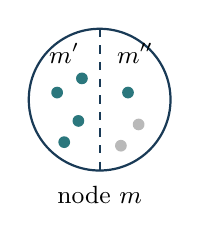
\begin{tikzpicture}[scale=0.9,
    p/.style={circle,fill=MyTeal,inner sep=1.5pt},
    o/.style={circle,fill=gray!55,inner sep=1.5pt}]
    \draw[MyNavy,thick] (0,0) circle (1.0);
    \draw[MyNavy,thick,dashed] (0,1.0) -- (0,-1.0);
    \node at (-0.5,0.65) {\small $m'$}; \node at (0.5,0.65) {\small $m''$};
    \node[p] at (-0.6,0.1) {}; \node[p] at (-0.3,-0.3) {};
    \node[p] at (-0.5,-0.6) {}; \node[p] at (-0.25,0.3) {};
    \node[p] at (0.4,0.1) {}; \node[o] at (0.55,-0.35) {};
    \node[o] at (0.3,-0.65) {};
    \node at (0,-1.35) {\small node $m$};
\end{tikzpicture}
\end{column}
\begin{column}{0.6\textwidth}
\small
\textbf{Co-located split:} $N' + N'' = N_m$, $D' + D'' = D(m)$, and
\[
f'(p\to q) = f\big(o(p)\to o(q)\big),
\]
where $o(\cdot)$ maps each piece back to $m$.
 
\vspace{0.1cm}
Pieces may have \emph{different} racial compositions.
\end{column}
\end{columns}
 
\begin{block}{Theorem (Splitting invariance)}
\begin{enumerate}
    \item[(a)] $\lambda^B = \lambda$;
    \item[(b)] $\hat s^B_{m'} = \hat s^B_{m''} = \hat s_m$, and
    $\hat s^B_p = \hat s_p$ for every untouched node $p$.
\end{enumerate}
\end{block}
% SAY: The index is per-person, so it is copied, not divided:
%      NOT s_m' + s_m'' = s_m. (Totals N * s still add up.)
\end{frame}
 
% ---------------------------------------------------------------------
% 11. The proof: one frame, three overlays (one navigation dot)
% ---------------------------------------------------------------------
\begin{frame}[shrink=0]
\frametitle<1>{Proof, Step 1: The Split Does Not Change the Walk}
\frametitle<2>{Proof, Steps 2--3: Survival Copied, Average Unchanged}
\frametitle<3>{Proof, Step 4: Read Off the Index}
 
\only<1>{%
\textbf{Normalizer.} For any node $p$ after the split, every old node
contributes as before, and the two pieces together contribute
\[
f\big(o(p)\to m\big)\,D' + f\big(o(p)\to m\big)\,D''
= f\big(o(p)\to m\big)\,D(m),
\]
exactly node $m$'s old term. So $Z'_p = Z_{o(p)}$.
 
\vspace{0.1cm}
\textbf{Kernel.} With co-location, for any two people $p, q$,
\[
K'(p,q) = \frac{f'\big(\ell'(p)\to\ell'(q)\big)}{Z'_{\ell'(p)}}
= \frac{f\big(\ell(p)\to\ell(q)\big)}{Z_{\ell(p)}} = K(p,q).
\]
\textbf{Killing} depends only on the race of the person drawn: unchanged.
 
\begin{block}{Conclusion}
Before and after the split, the walk $(X_t)$ and the killing time $T$
are the \emph{same random objects}. Only the node label written next to
each person changes: $L_t = \ell(X_t)$ becomes $L'_t = \ell'(X_t)$.
\end{block}
% SAY: Same people, same weights, same walk. This is the whole reason
%      for the invariance; the rest is bookkeeping.
}% end overlay 1
 
\only<2>{%
\textbf{Step 2: survival is copied.} By the backward equation,
$\sigma_i(n) = \Pr(T > n \mid X_0 \text{ at } i)$ under \emph{either}
labeling. Take a race-$r$ person $q$ in piece $m'$:
\[
\sigma^B_{m'}(n) = \Pr(T > n \mid X_0 = q) = \sigma^A_m(n),
\]
and the same for $m''$. Untouched nodes: $\sigma^B_p(n) = \sigma^A_p(n)$.
 
{\small Survival belongs to the person, and the person did not change.}
 
\vspace{0.15cm}
\textbf{Step 3: the average person is unchanged.}
\[
\bar\sigma^B(n)
= \frac{\sum_{p \ne m} N_p\,\sigma_p(n) + N'\sigma_m(n) + N''\sigma_m(n)}
       {\sum_{p \ne m} N_p + N' + N''}
= \bar\sigma^A(n),
\]
since $N' + N'' = N_m$ in both numerator and denominator.
 
{\small A node average would divide by $d+1$ instead of $d$:
the same people, counted differently.}
}% end overlay 2
 
\only<3>{%
\textbf{$B$ is primitive too.}
$B_{pq} = \dfrac{N_q}{N_{o(q)}}\, a_{o(p)o(q)}$: same zero pattern as $A$,
self-loops included. So the Corollary applies to $B$.
 
\vspace{0.15cm}
\textbf{Group index.}
\[
\lambda^B = \lim_{n\to\infty}\frac{\sigma^B_p(n+1)}{\sigma^B_p(n)}
\overset{\text{Step 2}}{=}
\lim_{n\to\infty}\frac{\sigma^A_{o(p)}(n+1)}{\sigma^A_{o(p)}(n)} = \lambda.
\]
\textbf{Individual index.}
\[
\hat s^B_p = \lim_{n\to\infty}\frac{\sigma^B_p(n+1)}{\bar\sigma^B(n)}
\overset{\text{Steps 2, 3}}{=}
\lim_{n\to\infty}\frac{\sigma^A_{o(p)}(n+1)}{\bar\sigma^A(n)}
= \hat s_{o(p)}. \qquad \blacksquare
\]
}% end overlay 3
\end{frame}
\section{Analysis}


\section{Normalizing The Metric}
%------------------------------------------------

%================================================
% SLIDE 1
%================================================
\begin{frame}[shrink=0]{Why normalize PSSI?}
\small

A larger group can have a higher raw score even when
it is more evenly distributed.

\medskip
\begin{columns}[T,onlytextwidth]

\begin{column}{0.48\textwidth}
\centering
\textbf{City A: 10\% group share}\\
All group members live in one neighborhood.

\medskip
\citydiagram{2}{0}{0.20}{0}

\[
    K_A=0.10,
    \qquad \boxed{\lambda_A=0.16}
\]
\end{column}

\begin{column}{0.48\textwidth}
\centering
\textbf{City B: 30\% group share}\\
The group is evenly distributed.

\medskip
\citydiagram{3}{3}{0.30}{0.30}

\[
    K_B=0.30,
    \qquad \boxed{\lambda_B=0.30}
\]
\end{column}

\end{columns}

\textbf{Goal:} Measure excess segregation relative to
a population-composition reference.

\medskip
{\footnotesize
Blue dots represent the studied group. Neighborhoods have equal
populations. Both cities use
$P=\left(\begin{smallmatrix}0.8&0.2\\0.2&0.8\end{smallmatrix}\right)$.
The raw score is
$\lambda=\rho(P\operatorname{diag}(r))$.
}

\end{frame}

%================================================
% SLIDE 2
%================================================
\begin{frame}[shrink=0]{PSSI as retention along an interaction path}
\small

Follow a random interaction path, stopping when it leaves
the studied group. Let $T$ denote the first exit time.

\begin{columns}[T,onlytextwidth]

\begin{column}{0.53\textwidth}
\centering
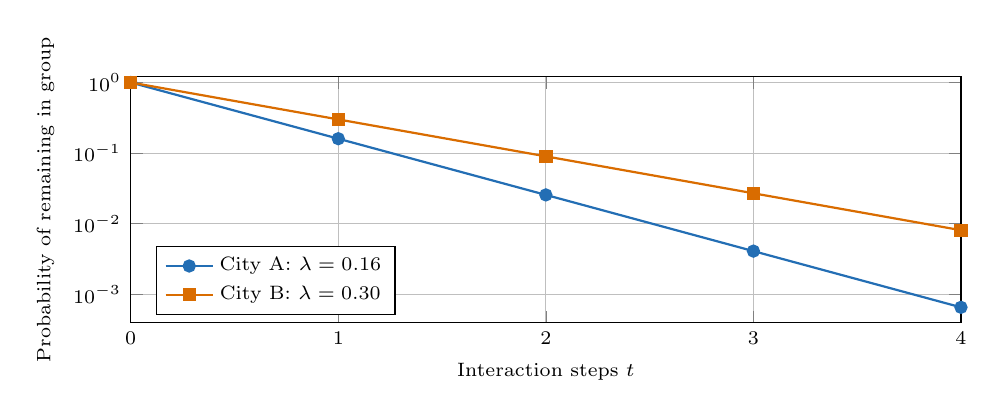
\begin{tikzpicture}
\begin{semilogyaxis}[
    width=\linewidth,
    height=4.7cm,
    xlabel={Interaction steps $t$},
    ylabel={Probability of remaining in group},
    xmin=0,xmax=4,
    ymin=0.0004,ymax=1.2,
    xtick={0,1,2,3,4},
    ytick={1,0.1,0.01,0.001},
    tick label style={font=\scriptsize},
    label style={font=\scriptsize},
    legend style={
        font=\scriptsize,
        at={(0.03,0.03)},
        anchor=south west
    },
    grid=major
]
\addplot[raceblue,thick,mark=*]
    coordinates {
        (0,1)
        (1,0.16)
        (2,0.0256)
        (3,0.004096)
        (4,0.00065536)
    };
\addlegendentry{City A: $\lambda=0.16$}

\addplot[orange!85!black,thick,mark=square*]
    coordinates {
        (0,1)
        (1,0.30)
        (2,0.09)
        (3,0.027)
        (4,0.0081)
    };
\addlegendentry{City B: $\lambda=0.30$}
\end{semilogyaxis}
\end{tikzpicture}

{\scriptsize
Exact survival probabilities for these examples,
starting with a uniformly chosen member of the studied group.
}
\end{column}

\begin{column}{0.44\textwidth}
\textbf{Conditional steady state}

For the within-group transition matrix $A$, a probability
row vector $q$ satisfying
\[
    qA=\lambda q
\]
obeys, when $\lambda>0$,
\[
    \frac{qA}{qA\mathbf{1}}=q.
\]
The location distribution among surviving paths stays
fixed, while each step retains a fraction $\lambda$.

\medskip
In these examples,
\[
    \Pr(T>t)=\lambda^t.
\]
City B retains more paths despite its uniform composition.
\end{column}

\end{columns}

\medskip
{\scriptsize
Matrix computation:
$A_A=\left(\begin{smallmatrix}0.16&0\\0.04&0\end{smallmatrix}\right)$,
$A_B=0.30P$.
Their spectral radii are $0.16$ and $0.30$.
For City A, $q=(1,0)$; for City B, $q=(1/2,1/2)$.
}

\end{frame}

%================================================
% SLIDE 3
%================================================
\begin{frame}[shrink=0]{Axiom 1: zero expected score under random mixing}
\small

Let $\Lambda$ be the raw score under a specified random-mixing
model, and write $m_0=\mathbb{E}_0[\Lambda]<1$.

\[
    \boxed{\mathbb{E}_0[\mu(\Lambda)]=0}
\]

\textbf{Why?}
A randomly mixed city should have adjusted score zero
on average, regardless of the group's population share.

\medskip
\textbf{A fast reference based on racial fraction}

For computation, we approximate the null mean by the citywide
racial fraction $K$:
\[
    m_0\approx K.
\]

\begin{itemize}
    \item This avoids repeated random-allocation simulations.
    \item It is exact for uniform local composition:
          $r_i=K$ gives $\rho(KP)=K$.
    \item At fixed $K$, the reference is independent of the graph.
          The observed score still responds to the city's
          spatial organization.
\end{itemize}

\medskip
{\footnotesize
Under a random-allocation model, $m_0$ can differ from $K$.
Using $K$ gives approximate null centering.
Graph invariance applies to the reference, not to the observed score.
}

\end{frame}

%================================================
% SLIDE 4
%================================================
\begin{frame}[shrink=0]{Axiom 2: a common upper reference}

\[
    \boxed{\mu(1)=1}
\]

\textbf{Why?}
Every racial group should use the same upper reference,
regardless of its population share.

\medskip
A raw score of one represents complete retention within
the group. Its normalized score should also equal one.

\medskip
\begin{itemize}
    \item Group size should not give one group a higher
          numerical ceiling than another.
    \item Zero at the baseline and one at the upper reference
          establish a common scale.
\end{itemize}

\medskip
{\footnotesize
The raw statistic lies in $[0,1]$ because
$\rho(P\operatorname{diag}(r))\leq
\max_i\sum_jP_{ij}r_j\leq1$.
One is a universal reference.
A fixed city's constraints may prevent it from attaining that value.
}

\end{frame}

%================================================
% SLIDE 5
%================================================
\begin{frame}[shrink=0]{Axiom 3: preservation of component averages}
\small

Suppose the studied group's interaction graph has two
disconnected sections.

\begin{center}
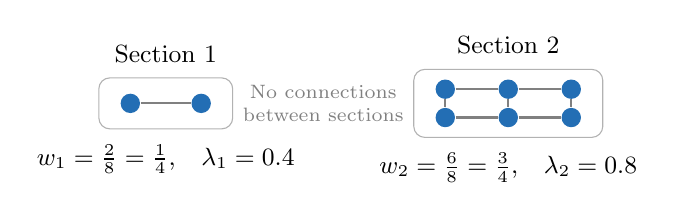
\begin{tikzpicture}[
    x=1cm,y=0.72cm,
    member/.style={
        circle,fill=raceblue,draw=none,
        minimum size=7pt,inner sep=0pt
    },
    edge/.style={gray,thick}
]
    \node[member] (a1) at (0,0) {};
    \node[member] (a2) at (0.9,0) {};
    \draw[edge] (a1)--(a2);

    \draw[rounded corners,gray!60]
        (-0.4,-0.45) rectangle (1.3,0.45);
    \node[above,font=\small] at (0.45,0.55)
        {Section 1};
    \node[below,align=center,font=\small] at (0.45,-0.55)
        {$w_1=\frac{2}{8}=\frac14$,\quad $\lambda_1=0.4$};

    \foreach \name/\x/\y in {
        b1/4/0.25,b2/4.8/0.25,b3/5.6/0.25,
        b4/4/-0.25,b5/4.8/-0.25,b6/5.6/-0.25
    }{
        \node[member] (\name) at (\x,\y) {};
    }

    \draw[edge] (b1)--(b2)--(b3);
    \draw[edge] (b4)--(b5)--(b6);
    \draw[edge] (b1)--(b4);
    \draw[edge] (b2)--(b5);
    \draw[edge] (b3)--(b6);

    \draw[rounded corners,gray!60]
        (3.6,-0.6) rectangle (6,0.6);
    \node[above,font=\small] at (4.8,0.7)
        {Section 2};
    \node[below,align=center,font=\small] at (4.8,-0.7)
        {$w_2=\frac{6}{8}=\frac34$,\quad $\lambda_2=0.8$};

    \node[align=center,text=gray,font=\scriptsize]
        at (2.45,0)
        {No connections\\between sections};
\end{tikzpicture}
\end{center}

Echenique and Fryer average component scores by group population:
\[
    S=w_1\lambda_1+w_2\lambda_2
      =\tfrac14(0.4)+\tfrac34(0.8)=0.7.
\]
We want the normalized score to preserve these weights:
\[
    \underbrace{\mu(0.7)}_{\text{Aggregate, then normalize}}
    =
    \underbrace{\tfrac14\mu(0.4)+\tfrac34\mu(0.8)}
               _{\text{Normalize, then aggregate}}.
\]
For all scores and nonnegative weights summing to one,
\[
    \boxed{\mu\!\left(\sum_iw_i\lambda_i\right)
       =\sum_iw_i\mu(\lambda_i)}.
\]

{\scriptsize
Source: Echenique and Fryer (2007), Proposition 4.
Connections are schematic; scores are illustrative.
Use one common calibration for all components.
This component average differs from the global spectral radius,
which takes the maximum component score.
}

\end{frame}

%================================================
% SLIDE 6
%================================================
\begin{frame}[shrink=0]{The axioms determine a unique normalization}
\small

Fix the raw statistic and its null model, with
$m_0=\mathbb{E}_0[\Lambda]<1$.

\textbf{Step 1: weighted averages force an affine function.}

Since $\lambda=\lambda\cdot1+(1-\lambda)\cdot0$,
Axioms 2 and 3 imply
\[
    \mu(\lambda)
      =\lambda\mu(1)+(1-\lambda)\mu(0)
      =\lambda+(1-\lambda)b,
    \qquad b=\mu(0).
\]

\textbf{Step 2: zero null expectation fixes the remaining constant.}

Axiom 1 gives
\[
    0=m_0+(1-m_0)b
    \quad\Longrightarrow\quad
    b=-\frac{m_0}{1-m_0}.
\]
Thus every admissible normalization must equal
\[
    \boxed{\displaystyle
       \mu(\lambda)=\frac{\lambda-m_0}{1-m_0}}.
\]

\textbf{Existence:} This formula preserves weighted averages,
has null expectation zero, and maps one to one.
Hence the normalization exists and is unique.

\medskip
{\footnotesize
With the computational reference $K<1$, use
$\mu_K(\lambda)=(\lambda-K)/(1-K)$.
For the illustrated cities:
$\mu_K(0.16)\approx0.067$ and $\mu_K(0.30)=0$.
The uniqueness theorem concerns a fixed raw statistic and null model.
\par\smallskip
Related normalization: Coleman's (1958) inbreeding-homophily index
$(H-K)/(1-K)$;
\href{https://doi.org/10.17730/humo.17.4.q5604m676260q8n7}{source}.
Here we apply chance adjustment to the spectral score.
}

\end{frame}

%================================================
% SLIDE 7
%================================================
\begin{frame}[shrink=0]{Further analysis: graph structure changes the null mean}
\small

Consider two neighborhoods with two residents each.
Randomly assign two group labels among the four residents:
$K=1/2$.

\begin{columns}[T,onlytextwidth]

\begin{column}{0.47\textwidth}
\textbf{Equal interaction across neighborhoods}
\[
    P_{\mathrm{mix}}=
    \begin{pmatrix}
        1/2&1/2\\
        1/2&1/2
    \end{pmatrix}.
\]
Every allocation gives
\[
    \lambda=\frac{r_1+r_2}{2}=\frac12.
\]
Therefore,
\[
    \boxed{m_{0,\mathrm{mix}}=\frac12}.
\]
\end{column}

\begin{column}{0.49\textwidth}
\textbf{Interaction within neighborhoods only}
\[
    P_{\mathrm{local}}=I,
    \qquad
    \lambda=\max(r_1,r_2).
\]
Both labels are in the same neighborhood with probability
$1/3$, and in different neighborhoods with probability $2/3$:
\[
    \boxed{
    m_{0,\mathrm{local}}
      =\frac13(1)+\frac23\left(\frac12\right)
      =\frac23}.
\]
\end{column}

\end{columns}

\medskip
The $K$ normalization then has expected null scores
\[
    \mathbb E_0[\mu_K(\Lambda_{\mathrm{mix}})]=0,
    \qquad
    \mathbb E_0[\mu_K(\Lambda_{\mathrm{local}})]=\frac13.
\]

\textbf{Interpretation:}
Using $m_0(P)$ adjusts for random allocation on each graph.
Using $K$ retains graph effects relative to a common reference.

\medskip
{\scriptsize
Exact counterexample for the global spectral-radius statistic.
Graph-independent calibration need not give exact null centering.
}

\end{frame}

%================================================
% SLIDE 8
%================================================
\begin{frame}[shrink=0]{Statistical test: is the $K$ approximation accurate enough?}
\small

Hold the graph, neighborhood populations, and total group count
fixed. Generate $B$ independent random allocations:
\[
    \Lambda_1,\ldots,\Lambda_B,
    \qquad
    \widehat m_0=\frac1B\sum_{b=1}^{B}\Lambda_b.
\]

The expected adjusted-score bias from using $K$ is
\[
    \boxed{
    \delta=\mathbb E_0[\mu_K(\Lambda)]
           =\frac{m_0-K}{1-K}}.
\]
Estimate this bias and its Monte Carlo standard error by
\[
    \widehat\delta=\frac{\widehat m_0-K}{1-K},
    \qquad
    \widehat{\operatorname{SE}}(\widehat\delta)
      =\frac{s_\Lambda}{(1-K)\sqrt B}.
\]

\textbf{Practical equivalence test}

Choose a tolerable error, such as $\varepsilon=0.02$.
Using the large-sample approximation, conclude equivalence at
the 5\% level if the 90\% confidence interval for $\delta$
lies entirely inside $[-\varepsilon,\varepsilon]$.

\medskip
\textbf{Suggested figure:}
Plot $\widehat\delta$ and its confidence interval against $K$,
separately for different graph structures.

\medskip
{\scriptsize
This tests approximation error, rather than treating a failure
to reject $m_0=K$ as evidence that the approximation is accurate.
Use the same raw-statistic definition in every simulation.
}

\end{frame}

%================================================
% SLIDE 9
%================================================
\begin{frame}[shrink=0]{A model where normalization recovers segregation exactly}
\small

Suppose the probability of remaining in the studied group is
\[
    p_{\mathrm{same}}=K+s(1-K),
    \qquad 0\leq s\leq1.
\]

Here $s$ measures the fraction of the gap between random mixing
and complete retention that has been closed.

\begin{itemize}
    \item $s=0$: same-group retention equals the racial fraction $K$.
    \item $s=1$: every interaction remains within the group.
\end{itemize}

If every row of the within-group transition matrix has this
same sum, then
\[
    \lambda=K+s(1-K).
\]
Consequently,
\[
    \boxed{
    \mu_K(\lambda)
      =\frac{K+s(1-K)-K}{1-K}
      =s}.
\]

\textbf{Simulation test:}
Hold $s$ fixed and vary $K$. Repeat with heterogeneous
neighborhoods and different interaction graphs.

\medskip
\textbf{Suggested figure:}
Plot adjusted score against $K$ for each fixed $s$.
Horizontal curves indicate population-share invariance
under the chosen model.

\end{frame}

%================================================
% SLIDE 10
%================================================
\begin{frame}[shrink=0]{Statistical significance and sensitivity}
\small

\textbf{Is the observed score unusually high?}

Under the specified random-allocation null, use
\[
    p=\frac{
        1+\sum_{b=1}^{B}
        \mathbf{1}\{\Lambda_b\geq\lambda_{\mathrm{obs}}\}
    }{B+1}.
\]
For a common baseline $m<1$, normalization is increasing:
\[
    \mu_m(\Lambda_b)\geq\mu_m(\lambda_{\mathrm{obs}})
    \iff
    \Lambda_b\geq\lambda_{\mathrm{obs}}.
\]
Thus normalization leaves this one-sided randomization
$p$-value unchanged.

\medskip
\textbf{How sensitive is the adjusted score?}
\[
    \frac{\partial\mu_m}{\partial\lambda}
      =\frac1{1-m},
    \qquad
    \frac{\partial\mu_m}{\partial m}
      =-\frac{1-\lambda}{(1-m)^2}.
\]
Errors can be amplified when the baseline is close to one.
Moreover,
\[
    \operatorname{Var}_0(\mu_m(\Lambda))
      =\frac{\operatorname{Var}_0(\Lambda)}{(1-m)^2}.
\]

\textbf{Reporting:}
Pair the normalized score with its randomization $p$-value.
Equal adjusted scores need not be equally unusual across cities.

\medskip
{\scriptsize
Monte Carlo $p$-value convention:
\href{https://docs.scipy.org/doc/scipy/reference/generated/scipy.stats.permutation_test.html}
{SciPy permutation-test documentation}.
The same calibration must apply to observed and simulated scores.
}

\end{frame}

\end{document}

